\chapter{Requirements}
\begin{figure}[h!]\centering
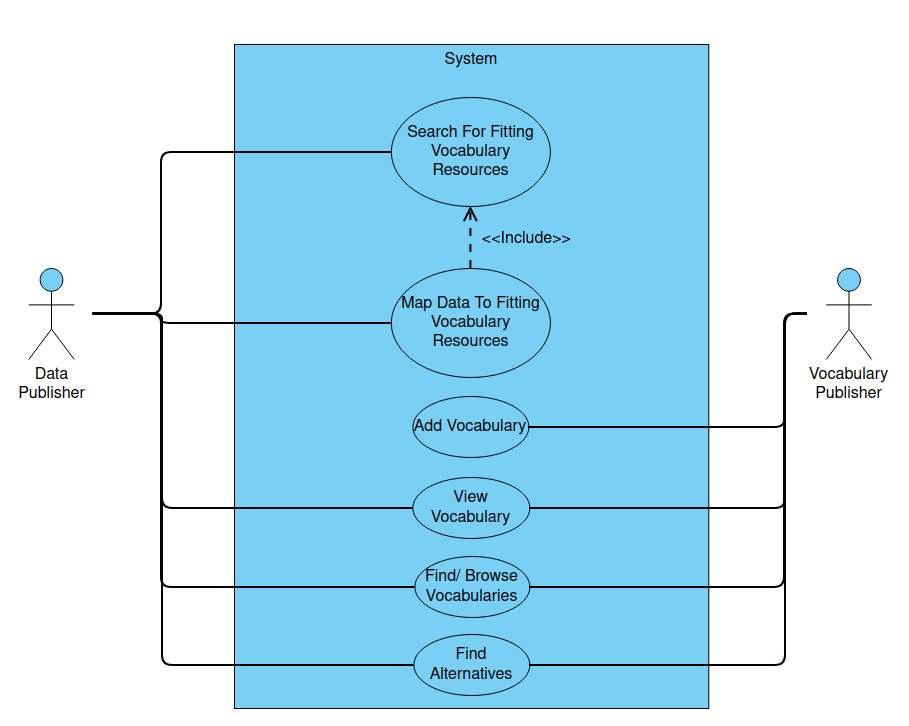
\includegraphics[width=120mm, height=120mm]{../img/use-case-diagram.png}
\caption{Use Case Diagram}
\label{fig:use-case}
\end{figure}                            
\section{Search For Fitting Vocabulary Resources}
\label{sec:fit-vocab-res}

\subsection{Description}
User has a conceptual model of some data. The user would like to find the best vocabulary resources to fit the data. User presents a graph of entitySets and their relations. The user can also specify other search parameters such as what predicates to consider for matching entitySets or which domain the data come from. The system returns a best-effort mapping options of vocabulary resources and predicates to specified entitySets and relationships between them. The user can then select the most fitting option or change the input specification to make the system search again.

The system tracks the last inputs and outputs so user does not have to repeat the search again if they want to go back. 

\subsection{Input}
The specification of entitySets and relationships within the input graph can be done multiple ways:
\begin{itemize}
    \item Provide string tags describing an entitySet or a relation.
    \item Provide already defined resource (IRI) as a final result value which stays in the result.
    \item Provide already defined resource (IRI) as a hint from which to gather tags.
    \item Provide placeholder relation or entitySet which can be matched by anything.
\end{itemize}

The system contains default rules for mapping entitySets and relations. The user can remove some rules or add more. Rules typically specify what general descriptive propertySets are used for tag matching or how different the output model can be from the input one. The rule can be specified for all entitySets or for any one entitySet. User can also indicate which domains the vocabularies should not be about so they can be filtered out beforehand or whether to search through all vocabularies.

\subsection{Output}
The output should provide the most fitting mappings for the input graph of entitySets and resources.

\section{Map Data To Fitting Vocabulary Resources}
\subsection{Description}
User can upload their RDF data and specify which resources and predicates should a mapping to vocabulary resources be found for. The system generates annotations which can be used as an input to the resource search described above in \autoref{sec:fit-vocab-res} to find the most fitting vocabulary resources to fit the data. The user can also provide the annotations. The user then either selects one of the found options or provides more hints to the system so it can find better results. If option is selected, the system produces the necessary triples so that the original data match the resulting resources.

\subsection{Input}
The input is RDF data in N-Quads or JSON-LD format. Same RDF things which fit under one logical class must have a class and belong to the same class so that the system can identify which RDF things represent the same concepts. (Or potentially let user load a conceptual model along with the data?)

User can specify which entitySets and predicates the mapping is found for via UI. Additionaly, any input for \autoref{sec:fit-vocab-res} can be added for customization of the mapping search.

\subsection{Output}
The output are triples which make the specified RDF things and predicates the found vocabulary classes. 

\section{Visualize Vocabulary And Its Resources}
\subsection{Description}
The system provides visualization for registered vocabularies. The visualization has two main components. One is a graph representation with entitySets as nodes and predicates as edges. User is able to navigate to the definition of entitySets and predicates via clicking on their representation in graph. The system also provides a definition for each entitySet which includes a list of all predicates along with their objects. User can view both predicates and objects by clicking on them. Predicate definitions contain any predicates made about them.

\section{Register Vocabulary}
\subsection{Description}
User can specify a vocabulary reference which is included in the system's vocabulary registry. User selects categories which the vocabulary fits in. The system also tries to find matching categories.

\section{Find Alternatives} 
\subsection{Description}
User searches for a similar resource to their defined resource. The systems does so by using same as links or comparing labels and resource's predicate labels. The system also lets user specify which predicates can be used for comparison.

\section{Browse Vocabularies}
\subsection{Description}
User can search for a vocabulary by specifying domain categories which should the vocabulary contain. The system provides a list of the most matchable vocabularies along with a summary of the most linked resource labels.



